% MPI performance

% 1. models 
% 1.1 Amdahl's law
% 1.2 Gustafson's law
% 2 Performance limiters
% 2.1 Local CPU performance
% 2.2 NIC bottleneck
% 2.3 Network cross section
% 3. Scaling studies
% 3.1 12 ways to fool the masses
% 3.2 strong scaling (Amdahl)
% 3.3 weak scaling (Gustafson)
% 4. top 500 supercomputers

Thus far in the course we have focused on capability, i.e. being able to write code that can run multi-threaded on shared memory systems with OpenMP and in parallel on a (possibly) distributed system with MPI. In the former we split work amongst threads that collaborate using shared system memory and in the latter separate processes collaborate on a task by exchanging data in messages. 

The question we must ask though: how effective is parallel computing ? In an ideal world if we use $P$ processors we would (maybe na\"{i}vely) expect the task to be completed $P$ times faster\footnote{Processors scales (rather nonlinearly) with the number of cores, their clock frequency, their fast memory cache capabilities, and their overall efficiency. More parallelism costs more money.}. If we define $T_P$ as the time it takes $P$ processors to complete a fixed task then we are expecting a ``speed up'', which we will denote by this formula
\[
S_P = \frac{T_1}{T_P},
\]
as the ratio of the task completion time for one processor over the task completion time for $P$ processors. We note immediately $S_1=1$ by definition. If indeed $P$ processors were to reduce the compute time by a factor of $P$ then $S_P=\frac{T_1}{T_1/P}=P$. In this lecture we will see that this is likely over optimistic and in practical calculations we may see significantly less than $P$ times speed up. 

\section{Amdahl's law}

In this section we consider an abstract model for a fixed task that is made parallel using $P$ processors. This model was first discussed by \href{https://en.wikipedia.org/wiki/Gene_Amdahl}{Gene Amdahl} at a computing conference in 1967 with a sketched discussion in proceedings \cite{amdahl1967validity}\footnote{Assignment: read and digest the paper by Amdahl}. According to \href{https://scholar.google.com/scholar?hl=en&as_sdt=0%2C47&q=amdahl%27s+law&btnG=}{scholar.google.com} there are now over 5000 articles that reference Amdahl's law despite the original description lacking a formal prescription for the ``law''.  

The main idea of the model is to assume that for every calculation there is a part of the task that cannot benefit from using more processors, which we will refer to as the ``serial fraction'' of the task denoted by $s\in[0,1]$. The model further assumes that the remainder of the task, or the ``parallel fraction'', can be performed with perfect parallel efficiency. 

In Amdahl's model the time that $P$ processors take to complete the task is assumed to be
\[
T_P = sT_1 + \frac{1-s}{P}T_1.
\]
In words the time it takes $P$ processes to complete the tasks consists of the time it takes one processor to complete the serial part of the task plus the time it takes $P$ to complete the remaining part of the task that is perfectly parallel.

The parallel speed up for this model is thus
\[
S_P = \frac{T_1}{T_P} = \frac{T_1}{sT_1 + \frac{1-s}{P}T_1} = \frac{1}{s + \frac{1-s}{P}}.
\]
{\bf Note}: Amdahl model speed up is relative and independent $T_1$. 

There are some interesting limits for the Amdahl speed up:
\begin{itemize}
 \setlength{\itemsep}{-4pt}
    \item $s=0$: in the case of a perfectly parallelizable task with no serial bottleneck the speed up is $S_P=P$.
    \item $s=1$: in the case of a purely serial task the speed up is $S_P=1$.
    \item $s=0.5$: when half the task is serial then the speed up approaches 2 from below as $P\rightarrow\infty$. Plainly speaking that you can throw as many processors at the task as you like, on the largest computer in the world, and you only get a factor of 2 speed up!
    \item $s=0.1$: if only ten percent of the task is bound to be serial then the maximum speed up you can get is ten!
    \item $s=0.01$: if only one percent of the task is serial you can still only get up to 100 times speed up. It doesn't matter if you use a computer with a thousand processors or even a million processors your code can only run a hundred times faster.
\end{itemize}

In Figure \ref{amdahl.fig} we plot the speed up curves for a range of different serial fractions. It should be striking that if only one percent of your computational task is bound to be serial then the best you can expect is a hundred times speed up. With that in mind you might wonder why equip the \href{https://www.olcf.ornl.gov/summit/}{Summit supercomputer} with over 27,000 GPUs that each in turn has 2560 floating point units ? That system can process a task with in excess of 70 million processing elements. By Amdahl's law we would require that a tiny fraction of the task be serial to fully utilize the Summit system. 

\begin{figure}[htbp!]
\begin{center}
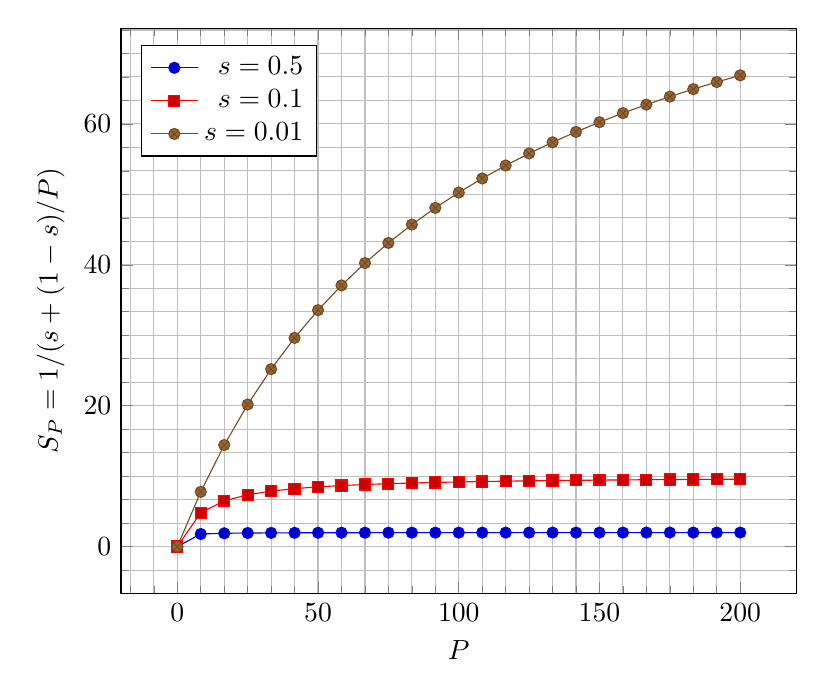
\begin{tikzpicture}
	\begin{axis}[
		xlabel=$P$,
		ylabel={$S_P = 1/(s+(1-s)/P)$},
		domain=0:200,
		legend style={
		    cells={anchor=east},
		    legend pos=north west,
	    },
	    width=4in,
	    grid=both,
	    minor tick num=5,
	]
	% use TeX as calculator:
	    \addplot {x/(0.5*x+0.5)};
	    \addlegendentry{$s=0.5$}
	    \addplot {x/(0.1*x+0.9)};
	    \addlegendentry{$s=0.1$}
	    \addplot {x/(0.01*x+0.99)};
	    \addlegendentry{$s=0.01$}
	\end{axis}
\end{tikzpicture}
\end{center}
\caption{Amdahl speed up $S_P$ for a range of serial fraction values.}
\label{amdahl.fig}
\end{figure}

In Figure \ref{amdahl2560.fig} we illustrate the dependence of the expected speed up for 2560 processors working for a fixed size problem as function of serial fraction. It is apparent that the parallel speed up drops off very quickly with even modest serial fraction.
\begin{figure}[htbp!]
\begin{center}
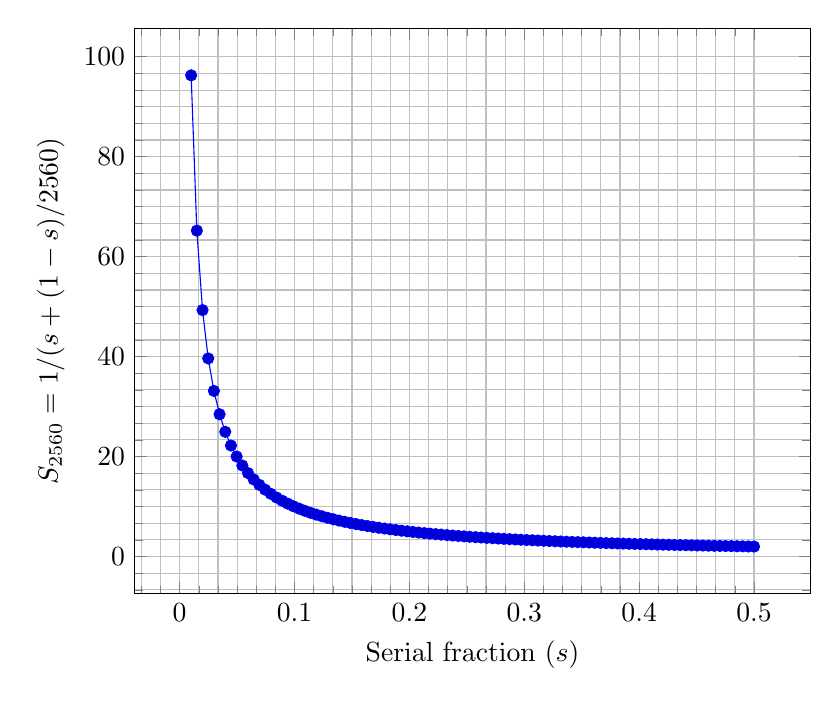
\begin{tikzpicture}
	\begin{axis}[
		xlabel={Serial fraction ($s$)},
		ylabel={$S_{2560} = 1/(s+(1-s)/2560)$},
		samples=100,
		domain=0.01:0.5,
		legend style={
		    cells={anchor=east},
		    legend pos=north west,
	    },
	    width=4in,
	    grid=both,
	    minor tick num=5,
	]
	% use TeX as calculator:
	    \addplot {1/(x + (1-x)/2560)};
	\end{axis}
\end{tikzpicture}
\end{center}
\caption{Amdahl speed up for $P=2650$ processors for a range of serial fraction values.}
\label{amdahl2560.fig}
\end{figure}


The fundamental issue here is that for a fixed size problems increasing $P$ drives the computational time for the parallel part of the problem to zero but does not change the time to compute the serial part.In the next section we introduce a less pessimistic model for parallel computing than Amdahl's parallel model. 

\section{Gustafson's law}

In 1988 John Gustafson revisited the doomsaying aspect of Amdahl's law \cite{gustafson1988reevaluating} for large scale parallel computing with many processors. Gustafson tweaked Amdahl's model by assuming that 

\begin{enumerate}
    \item The size of the problem grows in proportion to the number of processors (solve larger problems on larger systems).
    \item The serial fraction of the problem does not grow with increasing number of processors.
\end{enumerate}


In Gustafson's model the work performed by $P$ processors is
\[
W_P = sW_0 + P(1-s)W_0,
\]
which represents a fixed amount of serial work in the first expression and $P$ times the amount of the baseline parallelizable work $W_0$ for one processor.

The model parallel speed up will be the time it takes one processor to complete $W_P$ work divided by the time it takes $P$ processors to complete the work. Assuming that all processors complete work at the same rate, the speed up in this case is given by
\[
S_P := \frac{sW_0 + P(1-s)W_0}{sW_0 + \frac{P(1-s)W_0}{P}}.
\]
Simplifying this we get 
\[
S_P = s + (1-s)P.
\]
Thus we can expect the parallel speed up as defined above to be linear in the number of processors $P$ but with slope dictated by the parallel fraction. We only lose $sP$ in speed up relative to an optimal speed up. In Figure \ref{gustafson.fig} we illustrate the speed up estimate for a range of $P$ and serial fractions $s$.

\begin{figure}[htbp!]
\begin{center}
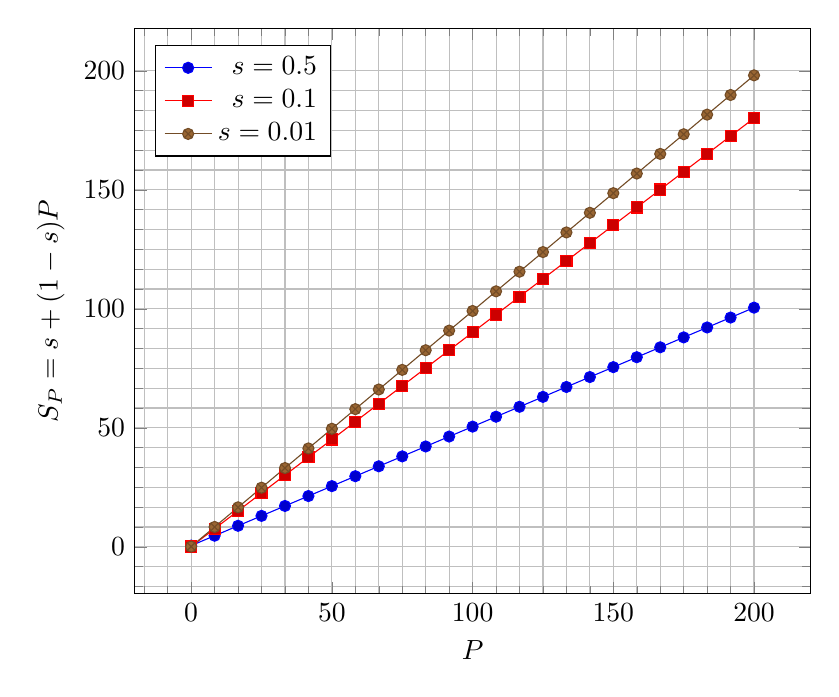
\begin{tikzpicture}
	\begin{axis}[
		xlabel=$P$,
		ylabel={$S_P = s+(1-s)P$},
		domain=0:200,
		legend style={
		    cells={anchor=east},
		    legend pos=north west,
	    },
	    width=4in,
	    grid=both,
	    minor tick num=5,
	]
	% use TeX as calculator:
	    \addplot {0.5 + (1-0.5)*x};
	    \addlegendentry{$s=0.5$}
	   \addplot {0.1 + (1-0.1)*x};
	    \addlegendentry{$s=0.1$}
	   \addplot {0.1 + (1-0.01)*x};
	    \addlegendentry{$s=0.01$}
	\end{axis}
\end{tikzpicture}
\end{center}
\caption{Gustafson speed up $S_P$ for a range of serial fraction values, assuming the parallel component of the computational task grows linearly with the processor count.}
\label{gustafson.fig}
\end{figure}

Gustafson's law is much less pessismistic than Amdahl's law. Following the logic we can better utilize the Summit system (or indeed the ARC cascades system) by increasing the problem size while also minimizing the serial component of the task to increase the slope of the speed up chart. The flip side of this analysis is that to fully occupy the 27,000+ GPUs on Summit we will need to solve problems that are 27,000 times larger than a single GPU can solve. 

\section{Conducting scaling studies}

In this section we describe how to conduct scaling studies, that is determining the speed up behavior of an MPI code as the number of MPI processes increases.

The first element of understanding how efficiently an MPI scales, that is how much speed up the code achieves when using $P$ processors is to accurately time the execution of the task in question. 

\subsection{MPI timing}

We rely on the MPI wall clock function \texttt{MPI\_Wtime} as a timing function, in much the same way as we used \texttt{omp\_get\_wtime} in OpenMP. Suppose we want to time how long an MPI reduction takes we will 
\begin{enumerate}
  \item Use \texttt{MPI\_Barrier} to make sure all MPI processes have finished prior tasks. 
  \item Then all processes will read the wall clock time with \texttt{MPI\_Wtime}, perform the MPI reduction \texttt{MPI\_Reduce} we wish to time, and then read the wall clock time again. 
  \item Each process will compute the time that elapsed during their participation in the \texttt{MPI\_Reduce} operation and to estimate the maximum time any process took in that function.
  \item Finally we use \texttt{MPI\_Allreduce} with the \texttt{MPI\_MAX} operation to reduce all of the computed max elapsed times from all processes into the global max time.
\end{enumerate} 

The following code provides two functions that provide a start timer and end timer that can be called before and after the piece of code you wish to time.

\begin{minted}{c}
double mpiStartTimer(){

  // make sure all MPI processes have completed prior tasks                                                                                                             
  MPI_Barrier(MPI_COMM_WORLD);

  // get start time                                                                                                                                                     
  return MPI_Wtime();
}

double mpiEndTimer(double start){

  // get wall clock end time                                                                                                                                            
  double end = MPI_Wtime();

  // find maximum elapsed time on any process                                                                                                                           
  int N = 1;
  double *message = (double*) calloc(N, sizeof(double));
  double *elapsed = (double*) calloc(N, sizeof(double));
  message[0] = end-start;
  MPI_Allreduce(message, elapsed, 1, MPI_DOUBLE, MPI_MAX, MPI_COMM_WORLD);

  double res = elapsed[0];
  free(elapsed);
  free(message);

  return res;
}
\end{minted}

With an example where we time how long it takes to add up the entries in a local array and then do a distributed MPI reduction operation to sum up all those local array sums.
\begin{minted}{c}
  int Nlocal = atoi(argv[1]);
  double *v = (double*) calloc(Nlocal, sizeof(double));

  for(int n=0;n<Nlocal;++n)
    v[n] = 1;

  // set up message buffer for reduction  
  int N = 1;
  double *message = (double*) calloc(N, sizeof(double));
  double *answer  = (double*) calloc(N, sizeof(double));

  // start timer =====================================> 
  double start = mpiStartTimer();

  // locally reduce array          
  double res = 0;
  for(int n=0;n<Nlocal;++n)
    res += v[n];
  message[0] = res;

  // perform distributed sum reduction   
  int root = 0; // destination for sum of distributed message entries                                                                           
  MPI_Reduce(message, answer, N, MPI_DOUBLE, MPI_SUM, root, MPI_COMM_WORLD);

  // compute elapsed time <==============================
  double elapsed = mpiEndTimer(start);

  if(rank==root)
    printf("%d %g %lf %%, computed\n", size, elapsed, answer[0]);
\end{minted}

When I run this code with 6 MPI processes and 10 million entries (of value one) in each local array I get the following

\myvbox[mytermbg]{mpiexec -n 6 ./mpiTimer 10000000 \\
6 0.0252972 60000000.000000 \%\% MPI size, elapsed, \\ computed
}

That is it took .025 seconds to complete the local work and the finishing global reduction. Repeating with 12 MPI processes on my workstation I get

\myvbox[mytermbg]{mpiexec -n 12 ./mpiTimer 10000000 \\
12 0.028229 120000000.000000 \%\% MPI size, elapsed,\\ computed
}

\section{Weak scaling study}

{\bf Weak scaling definition}: time how long it takes $P$ processes to complete a task that grows linearly with $P$ for a range of $P$. We then compare the time it would take one process to complete the scaled up task.

In the above code we increase the work with the number of ranks, since the number of entries being summed by each rank is fixed at 10 million. This type of scaling is called weak scaling and falls into the models described by Gustafson. In our results above the scaling is fairly reasonable since the time it took 12 processes is not a huge increase over the time it took 6 processes. In an ideal world the time would be the same but Gustafson predicts that the difference is due to some serial component of the calculation.

It is customary to test for a range of process counts and to plot the time it takes to complete the task. In Figure \ref{reductionWeakScalingStudy.fig} we show the timings for this weak scaling study. In an ideal world the time it takes one process should be the same as it takes two processes to complete the task. 
\begin{figure}[htbp!]
\begin{center}
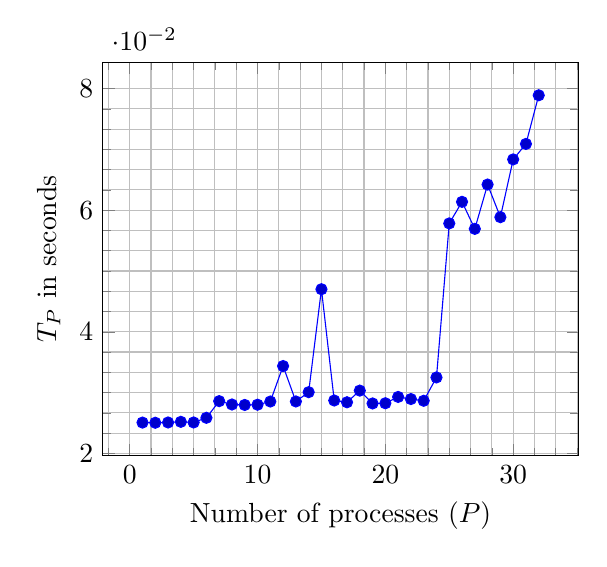
\begin{tikzpicture}
	\begin{axis}[
		xlabel={Number of processes ($P$)},
		ylabel={$T_P$ in seconds},
		domain=1:32,
		legend style={
		    cells={anchor=east},
		    legend pos=north west,
	    },
	    width=3in,
	    grid=both,
	    minor tick num=5,
	]
    \addplot coordinates {
(1, 0.0250647)
(2, 0.0250371)
(3, 0.0250821)
(4, 0.0251884)
(5, 0.0250831)
(6, 0.0258505)
(7, 0.0285928)
(8, 0.0280409)
(9, 0.0279655)
(10, 0.0280035)
(11, 0.0285277)
(12, 0.0343659)
(13, 0.0285378)
(14, 0.0300694)
(15, 0.0469997)
(16, 0.0286977)
(17, 0.0284054)
(18, 0.0303254)
(19, 0.0282125)
(20, 0.0282428)
(21, 0.0292845)
(22, 0.0289357)
(23, 0.0286508)
(24, 0.0324934)
(25, 0.0578246)
(26, 0.0613713)
(27, 0.0569243)
(28, 0.0642169)
(29, 0.0588481)
(30, 0.0683491)
(31, 0.0708976)
(32, 0.0788972)

};
	\end{axis}
\end{tikzpicture}
\end{center}
\caption{Weak scaling study: each process sums up 10 million entries in an array and then all processes participate in \texttt{MPI\_Reduce} to sum their values up. Experiment performed on workstation with two   Intel(R) Xeon(R) Gold 6128 CPU @ 3.40GHz processors. Each CPU has 6 cores and can hardware hyperthread with two threads per core.
 }
\label{reductionWeakScalingStudy.fig}
\end{figure}

Referring to Figure \ref{reductionWeakScalingStudy.fig} we see that instead of being flat there is some variation in $T_P$ up to $P=10$, some spikes between $P=11$ and $P=13$ and a major jump at $P=23$. The spikes are likely due to other processes on the workstation preempting the MPI processes. The major jump at $P=23$ corresponds to the saturation of all hardware threads on the CPU. 

We can reduce the variability due to OS noise by either increasing the number of times we run the experiment and averaging the results or running the experiment with a larger array. In Figure \ref{reductionWeakScalingStudy100.fig} we did the latter increasing the processor local arrays to 100 million doubles.  We do indeed see that the variability has diminished for small process counts. 

The experiments were performed on a workstation with two CPUs each equipped with 6 cores. Each core can perform hyperthreading, but as we see in the figure the time $T_P$ jumps by a factor of 2 at about $P=11$. Although the hyperthreading is effective it is something of a marketing gimmick by Intel.

\begin{figure}[htbp!]
\begin{center}
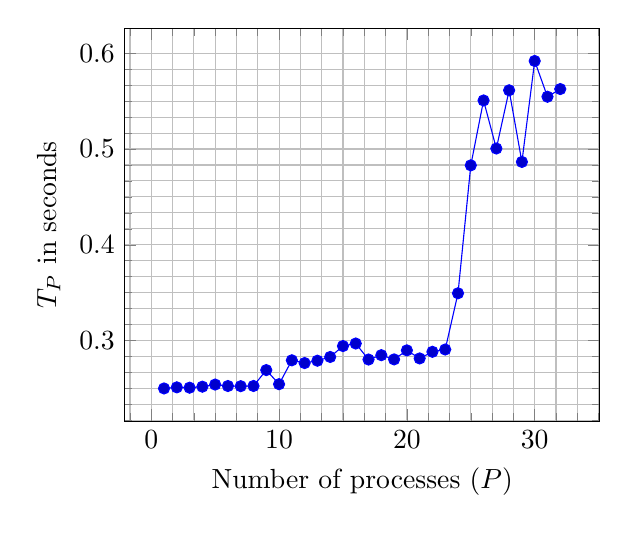
\begin{tikzpicture}
	\begin{axis}[
		xlabel={Number of processes ($P$)},
		ylabel={$T_P$ in seconds},
		domain=1:32,
		legend style={
		    cells={anchor=east},
		    legend pos=north west,
	    },
	    width=3in,
	    grid=both,
	    minor tick num=5,
	]
    \addplot coordinates {
(1, 0.249957)
(2, 0.251113)
(3, 0.250758)
(4, 0.251816)
(5, 0.254025)
(6, 0.252513)
(7, 0.252338)
(8, 0.252553)
(9, 0.269128)
(10, 0.25441)
(11, 0.279367)
(12, 0.276479)
(13, 0.278934)
(14, 0.282854)
(15, 0.294243)
(16, 0.296885)
(17, 0.280154)
(18, 0.284715)
(19, 0.280304)
(20, 0.289727)
(21, 0.281318)
(22, 0.288236)
(23, 0.290642)
(24, 0.349358)
(25, 0.482953)
(26, 0.550729)
(27, 0.500544)
(28, 0.561326)
(29, 0.486533)
(30, 0.591954)
(31, 0.554609)
(32, 0.562627)
};
	\end{axis}
\end{tikzpicture}
\end{center}
\caption{Weak scaling study: each process sums up 100 million entries in an array and then all processes participate in \texttt{MPI\_Reduce} to sum their values up. Experiment performed on workstation with two   Intel(R) Xeon(R) Gold 6128 CPU @ 3.40GHz processors. Each CPU has 6 cores and can hardware hyperthread with two threads per core.
 }
\label{reductionWeakScalingStudy100.fig}
\end{figure}

\section{Strong scaling study}

{\bf Strong scaling definition}: keep the problem size fixed and time how long it takes different number of processes to complete the task.

%% for P in `seq 1 6`; do mpiexec  -n $P ./mpiStrongScaling 10000000; done

We approach this systematically using bash shell magic to run \texttt{L21/mpiStrongScaling.c} on a compute node on cascades. First we use slurm alloc to grab a node with an allocation of 28 cores with

\myvbox[mytermbg]{salloc --partition=dev\_q --nodes=1 --tasks-per-node=28  -Acmda3634}

We next load the \texttt{openmpi} module 
\myvbox[mytermbg]{module load gcc openmpi}

Then we make sure the code is built
\myvbox[mytermbg]{cd cmda3634/L21/ \\ mpicc -o mpiStrongScaling mpiStrongScaling.c -lm}

The we use a bash for loop in the terminal to run the \texttt{mpiStrongScaling} executable with one to 28 processes
\myvbox[mytermbg]{for P in `seq 1 28`; \\ 
 \; do mpiexec  -n \$P ./mpiStrongScaling 10000000 |\& grep elapsed;\\ 
done}

We gather the output data and I plotted the time that the calculation takes for each $P$ in Figure \ref{strongScaling.fig}. Notice how it dips nicely down until abaout 22 processes then it shows some non-monotonic variation. For the large process count each process is competing with the OS and other processes for time on a core.
\boximagelabel{figures/L20/strongScalingCascades-crop.pdf}{Strong scaling study using \texttt{L21/mpiStrongScaling.c}}{strongScaling.fig}
Although it is reassuring that the time goes down with increasing process count, it is not very informative about the efficiency of our parallel code. In Figure \ref{strongSpeedupScaling.fig} we plot the speed up $S_P = T_1/T_P$ as a function of $P$. If the code scaled perfectly then the blue line would track the red reference line with speed up given by $P$. However, we see that the speed up deviates from perfect scalability as we would expect given Amdahl's analysis. With 28 processes we get about a 23 times speed up, not terrible but also not super!

\boximagelabel{figures/L20/strongScalingSpeedupCascades-crop.pdf}{Strong scaling speed up study using \texttt{L21/mpiStrongScaling.c}}{strongSpeedupScaling.fig}

In practice we observe that the timings become ``noisy''  as the core count per compute node increases. This is due to other processes running on the compute node. For modeling processes it is common practice (albeit walking close to the line for honest reporting \cite{bailey199112}) to run the task a number of times and use averaged timing data to eliminate outliers. This is done with a simple for loop as follows

\begin{minted}{c}
int Ntests = 100;

  // start timer =====================================> 
  double start = mpiStartTimer();

  for(int test=0;test<Ntests;++test){

    // locally reduce array
    double res = 0;
    for(int n=0;n<Nlocal;++n)
      res += v[n];
    message[0] = res;

    // perform distributed sum reduction 
    MPI_Reduce(message, answer, N, MPI_DOUBLE, MPI_SUM, root, MPI_COMM_WORLD);
  }

  // compute elapsed time <==============================
  double elapsed = mpiEndTimer(start)/Ntests;
\end{minted}

\section{Beyond Amdahl and Gustafson}

The models that were proposed by Amdahl and Gustafson are useful but limited in scope. Given a specific code we can add terms in the model for $T_P$ that match specific operations, or classes of operations. For instance we can model $T_P$ for the vector sum reduction task we used to measure strong scaling with a three term expression as follows
\[
T_P \approx T_1\left(s + p\frac{1}{P} + r\log_2(P)\right)
\]
where $s$ represents serial fraction, $p$ represents parallel fraction, and $r$ represents a new temporal contribution for the parallel MPI reduction operation. 

We measure $T_P$ for a range of process counts $P$ as before. We then use a least squares approximation to estimate the unknown coefficients $p,s,r$ for a specific scaling study with the following MATLAB code.

\begin{minted}{matlab}
%% purpose:
%% given an array of process numbers P, and times taken by those processes
%%   1. least squares fit the data to s + p/P + r*log2(P)
%%   2. reconstruct fit at pP
%%   3. plot original data and fit
function [a,pTP] = plotStrongScalingData(P, TP, pP)

  %% least squares fit to model:
  %% TP ~= s + p/P + r*log2(P) 
  M = [ones(size(P)),1./P, log2(P)];
  a = (M'*M)\(M'*TP);

  %% reconstruct fit at plotting points
  pTP = a(1) + a(2)./pP + a(3)*log2(pP);

  %% plot sampled data and reconstructed fit data
  plot(P,TP, 'ro', pP, pTP, 'b-')

  return
end
\end{minted}

In Figure \ref{advancedStrongScalingTime.fig} we show experimental data obtained running the \texttt{L21/mpiAdvancedStrongScaling.c} example code that performs a fixed size vector reduction 100 times and reports \underline{average} computational time $T_P$ for $P$ MPI processes. We ran with the following command choosing a smaller than usual problem to expose the existence of the serial component since the parallel work is relatively small.

\myvbox[mytermbg]{for P in `seq 1 20` \\  do \\  mpiexec -n \$P ./mpiStrongScaling 10000 |\& grep elapsed; \\done
}

\boximagelabel{figures/L20/advancedModelTimeReduction10000-crop.pdf}{Three term model fit for parallel execution time $T_P$ based on serial, parallel, and reduction components estimated through least squares fit of experimental dat measured on Cascades compute node using up to 20 processes performing a fixed global size vector reduction \texttt{L21/mpiAdvancedStrongScaling.c}}{advancedStrongScalingTime.fig}
Note that the computed fit (blue line) is a relatively good approximation to the measured data (red circles) up to 20 processes. Repeating with more data for larger $P$ introduces some spikes in the timing data even with averaged $T_P$ from a hundred test runs.

In Figure \ref{advancedStrongScalingSpeedup.fig} we represent the scaling study in terms of speed up. We see that the model does a good job of capturing the speed up. The least squares fit yields
\begin{eqnarray*}
s &=& 0.17,\\
p &=& 0.83,\\
r &=&-0.017.
\end{eqnarray*}
This suggests that the model is dominated for small $P$ by the regular Amdahl model terms. 

\boximagelabel{figures/L20/advancedModelSpeedupReduction10000-crop.pdf}{Three term model fit for parallel speed up $S_P=T_1/T_P$ based on serial, parallel, and reduction components estimated through least squares fit of experimental data measured on Cascades compute node using up to 20 processes performing a fixed global size vector reduction \texttt{L21/mpiAdvancedStrongScaling.c}}{advancedStrongScalingSpeedup.fig}.


The CPUs in the cascades nodes that we are using are the \href{https://ark.intel.com/content/www/us/en/ark/products/91766/intel-xeon-processor-e5-2683-v4-40m-cache-2-10-ghz.html}{Intel® Xeon® Processor E5-2683 v4} model. Each has 16 cores, and there are two of these CPUs per compute node (which are so-called ``dual socket'' nodes). Thus the node should be able to scale to 32 MPI processes. However, we start to see degradation of scaling at about 21 or 22 processes. This might be because other uses are running jobs on the same compute nodes, or it might be because of contention between our compute task and other operating system tasks. There also seem to be magic values of $P$ for which the spikes are less common than others. I am not sure what is causing that behavior ! Worse still to get the good fit we are guilty of ``cherry picking'' the process counts up to $P=20$ as using the results from higher process counts causes spikes that globally shift the model upwards and make the model lose accuracy for small $P$.




\section{Caveats: honesty in reporting and interpreting parallel performance results}

I recommend you read ``\emph{Twelve Ways to Fool the Masses When Giving Performance Results on Parallel Computers}'' by David H. Bailey \cite{bailey199112}. There are many ways to misrepresent parallel performance achieved by code and that article did a good job way back in 1991 of highlighting some nefarious reporting tendencies. While you read the article determine how many your instructor has been guilty of in this lecture !


\printbibliography[heading=subbibliography]
